\section{Results}

We present results for three major settings:
\begin{itemize}
    \item Performance of fully pre-trained large language models across different number of shots.
    \item Development of performance over the course of training on our pre-training datamix.
    \item Scaling laws ablations across different compute flops and seeds.
\end{itemize}

\subsection{Performance on fully trained models}

We first show performance of various fully pre-trained models across 5 tasks (ANLI, HANS NLI, MNLI, SNLI, and AbductiveNLI). From figures \ref{fig:anli} - \ref{fig:abductivenli}, we can observe that model performance is above random accuracy for all tasks. 0-shot performance is quite bad but the models quickly improve with 1-shot and then saturate after 3 or 4 shots. Additionally, there's a clear gap between model sizes (405B > 70B > 8B) except for AbductiveNLI, where the 70B and 405B models saturate around the same accuracy of 85\%.

\begin{figure}[t]
    \centering
    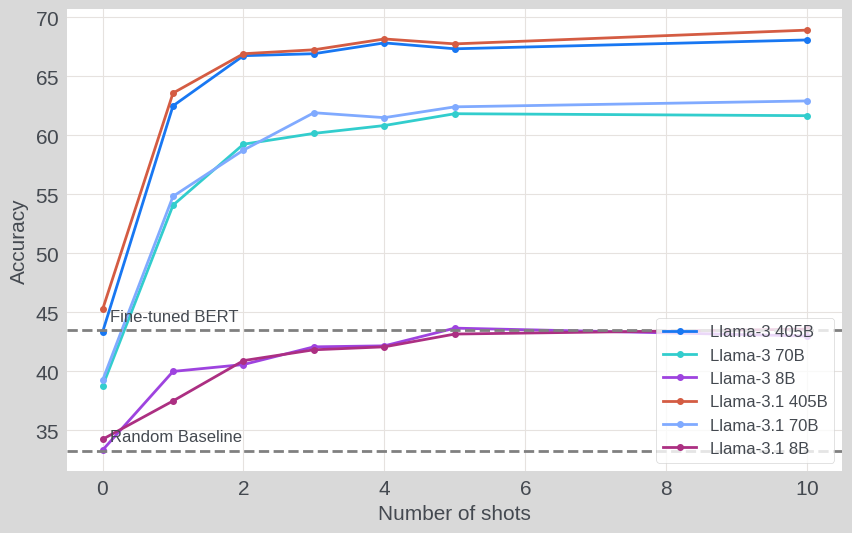
\includegraphics[width=0.45\textwidth]{nli_plots/anli.png}
    \caption{ANLI}
    \label{fig:anli}
\end{figure}

\begin{figure}[t]
    \centering
    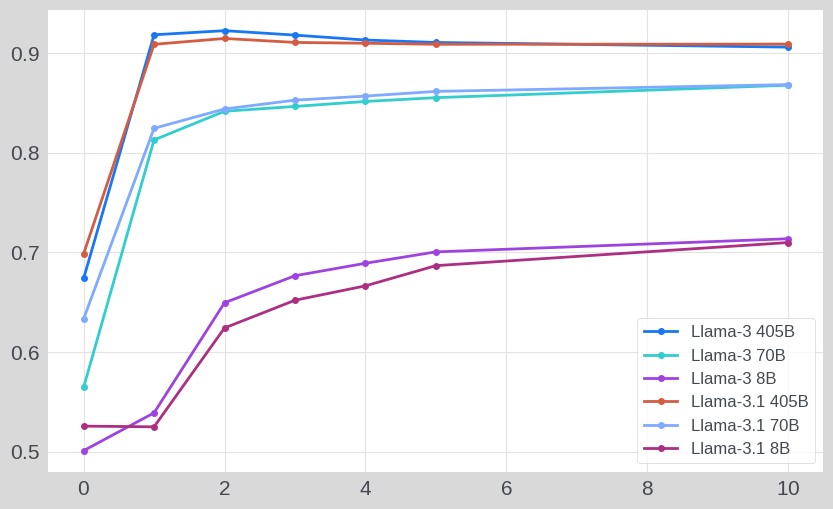
\includegraphics[width=0.45\textwidth]{nli_plots/hansnli.png}
    \caption{HansNLI}
    \label{fig:hansnli}
\end{figure}

\begin{figure}[t]
    \centering
    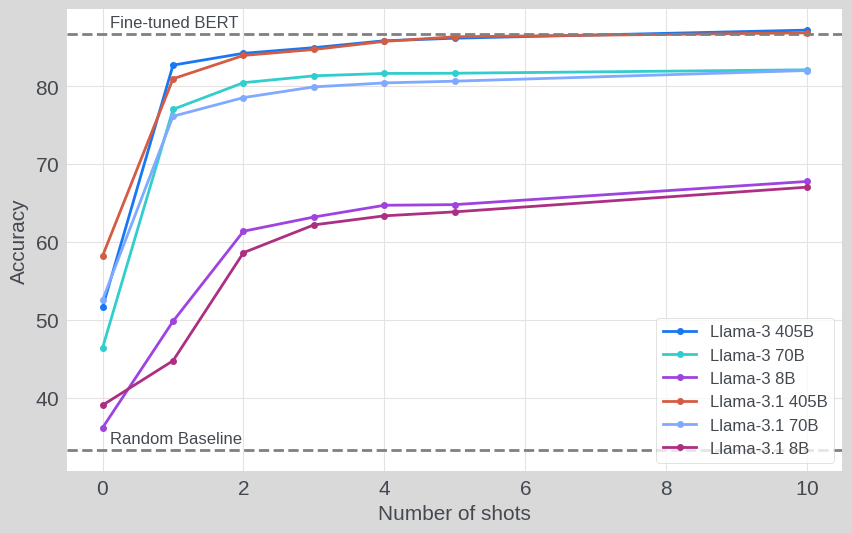
\includegraphics[width=0.45\textwidth]{nli_plots/mnli_matched.png}
    \caption{MNLI}
    \label{fig:mnli}
\end{figure}

\begin{figure}[t]
    \centering
    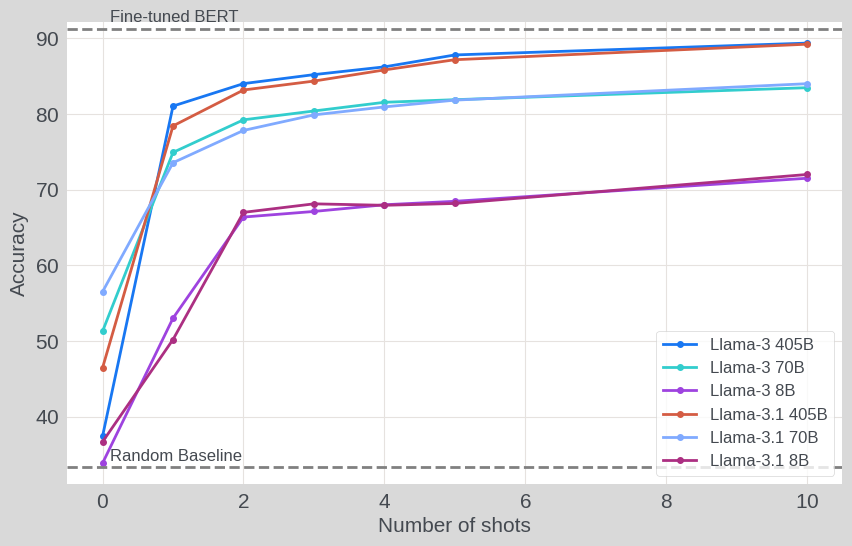
\includegraphics[width=0.45\textwidth]{nli_plots/snli.png}
    \caption{SNLI}
    \label{fig:snli}
\end{figure}

\begin{figure}[t]
    \centering
    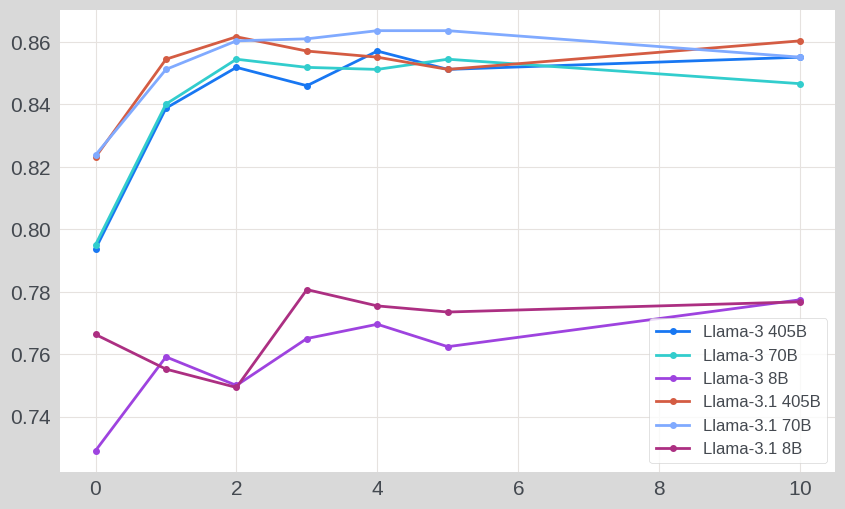
\includegraphics[width=0.45\textwidth]{nli_plots/abductivenli.png}
    \caption{AbductiveNLI}
    \label{fig:abductivenli}
\end{figure}

We also analyse the pre-training curves as shown in Figures \ref{fig:anli_int} - \ref{fig:abductivenli_int}.

\begin{figure}[t]
    \centering
    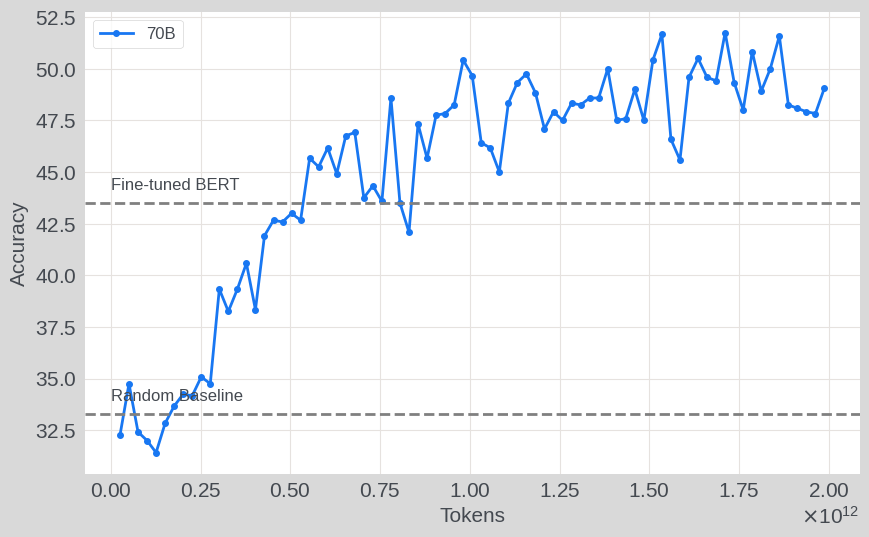
\includegraphics[width=0.45\textwidth]{nli_plots/anli_intermediate.png}
    \caption{ANLI}
    \label{fig:anli_int}
\end{figure}

\begin{figure}[t]
    \centering
    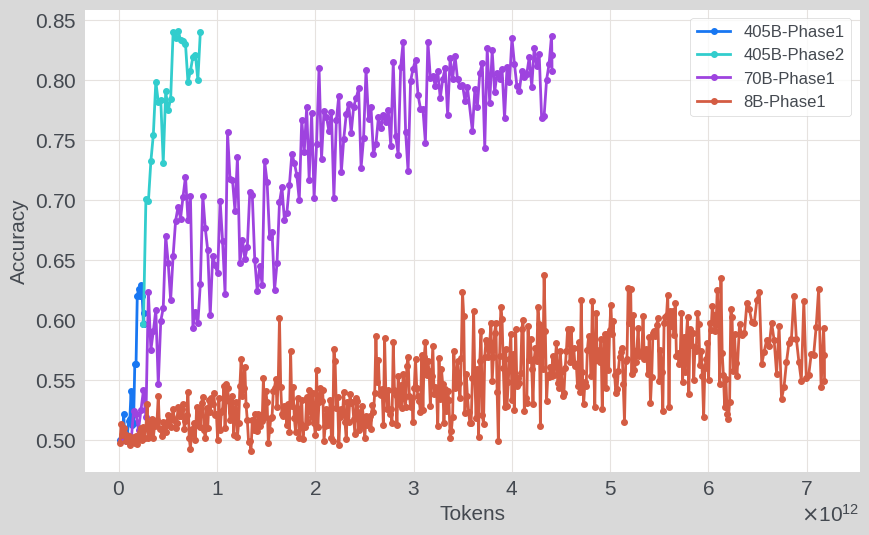
\includegraphics[width=0.45\textwidth]{nli_plots/hansnli_intermediate.png}
    \caption{HansNLI}
    \label{fig:hansnli_int}
\end{figure}

\begin{figure}[t]
    \centering
    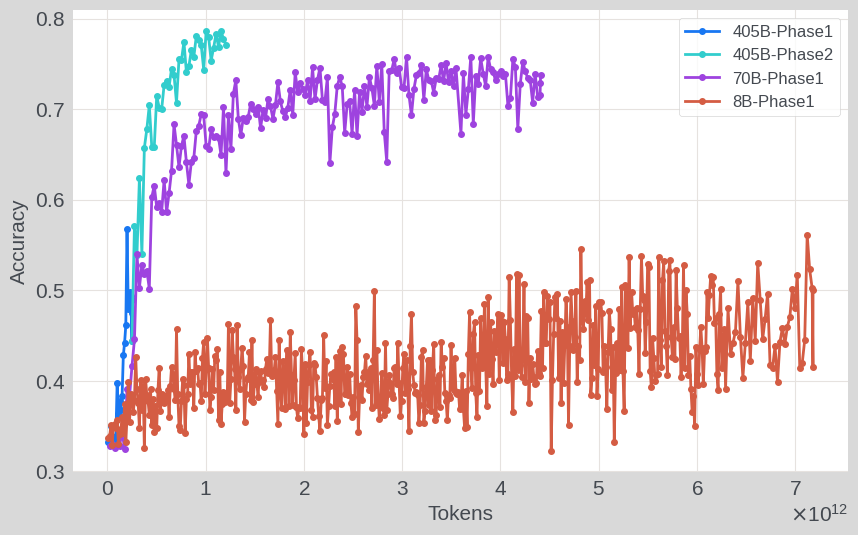
\includegraphics[width=0.45\textwidth]{nli_plots/mnli_matched_intermediate.png}
    \caption{MNLI}
    \label{fig:mnli_int}
\end{figure}

\begin{figure}[t]
    \centering
    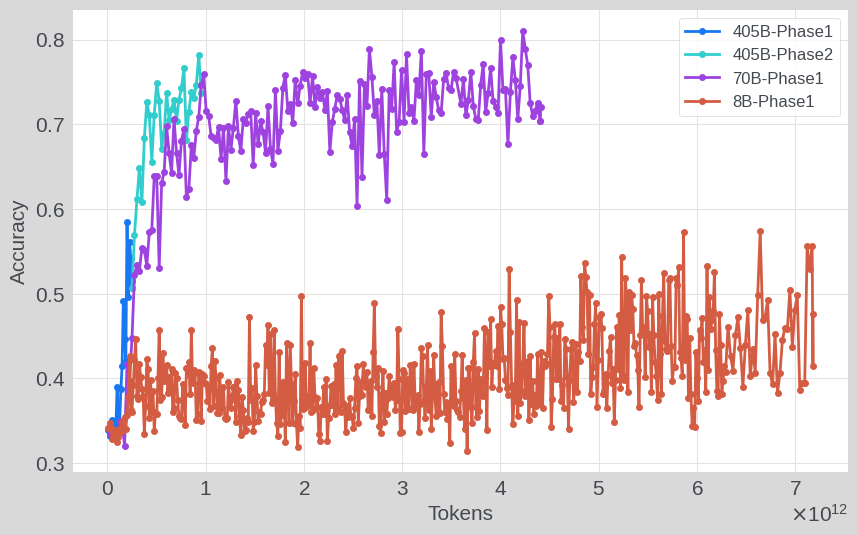
\includegraphics[width=0.45\textwidth]{nli_plots/snli_intermediate.png}
    \caption{SNLI}
    \label{fig:snli_int}
\end{figure}

\begin{figure}[t]
    \centering
    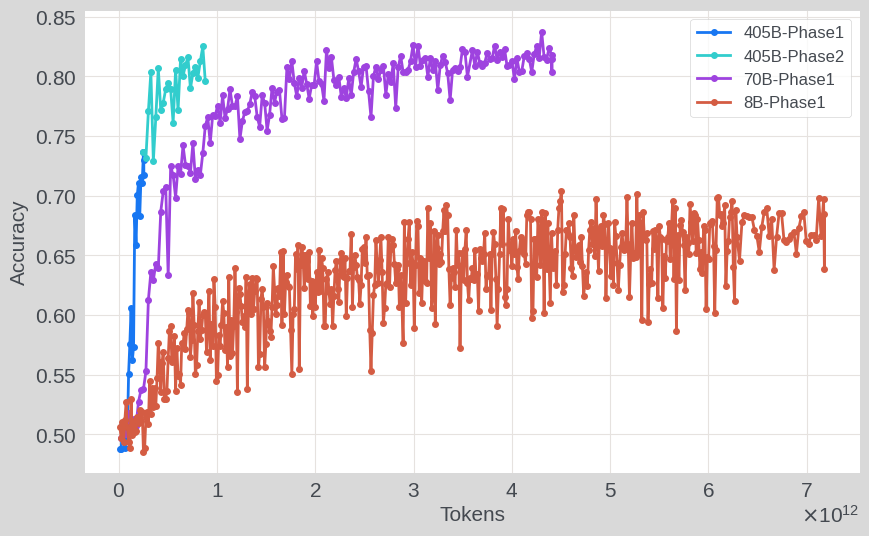
\includegraphics[width=0.45\textwidth]{nli_plots/abductivenli_intermediate.png}
    \caption{AbductiveNLI}
    \label{fig:abductivenli_int}
\end{figure}

\begin{figure*}[ht]
    \centering
    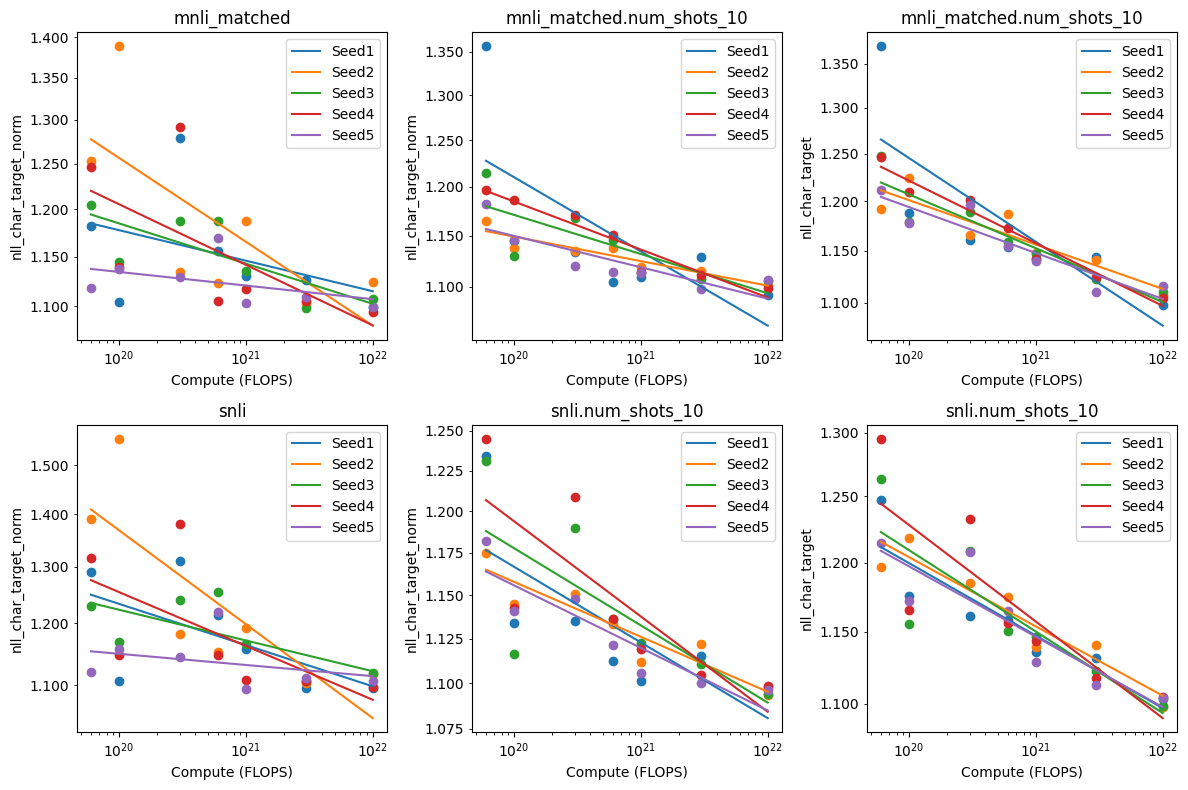
\includegraphics[width=0.95\textwidth]{nli_plots/sl_fits_mnli_snli.png}
    \caption{Scaling law curve fits across different compute FLOPs}
    \label{fig:sl_mnli_snli}
\end{figure*}

\paragraph{Q1: Does NLI provide signal for LLMs?}
We show \begin{enumerate}
    \item curves + scores on trained-out models.  Conclusion: ? Should say something about whether it is separating models in early stages of training, and whether it is monotonic, how much variance etc.
    \item Trained out model scores. Tentative conclusion (pending numbers): with the exception of abductive NLI, these datasets allow to distiguish models of different sizes. Doesn't work at all with zero-shot (which can explain some previous results?), but with one or two shots we get decent scores. ANLI seems to be the most challenging with around 70\% accuracy on the 405B model.
    \item Ablations: conclusion??
\end{enumerate}

NB: put contamination results somewhere.

Overall conclusion: seems to be useful both for training and trained-out models, an open question however is, is there still room to improve?

\paragraph{Q2: Is there still room for improvement?}
We do an light-weight manual analysis (e.g. check 20 examples).
Probable conclusion: there may be some errors, but oftentimes models make incorrect predictions on samples on which humans may disagree too.

To substantiate this claim, we consider chaosNLI.
We show 1) entropy plots for various models, these show that the larger models have pretty much perfect perfrmance on samples where humans agree across the board, but drop off on other examples. Smaller models don't get perfect performance also on the former. Results also show that a small amount of errors is due to annotation errors (or not matching majority labels), because the `corrected' accuracy is slightly higher than the non-corrected accuracy.
2) We show KL-divergence with human distributions. Conclusion: this gets better with scale (contradicts earlier findings!), but still far away from human alignment. Still room for improvement. We check how stable this signal is across training (so we show curves of KL/JSD and see whether this provides a astable signal.


% \begin{itemize}
%   \item Final pre-trained model result analysis. How model size, prompts, and shots affect things across various tasks.
%   \item Development of model performance for a given task across model sizes.
%   \item Correlation of model performance development with other commonsense/normal reasoning tasks (race, obqa, mmlu, math, etc.)
%   \item Results on ChaosNLI and how model scores relate to the distribution of human judgements. Model size/prompt analysis for this too.
%   \item Large models are good, but is it because of better models/training or just contamination? Contamination Analysis on various benchmarks.
%   \item Can NLI tasks help in pre-training ablations? Results on seed models and models trained on different datamixes. How does the effectiveness of a given dataset/datamix is affected under different datasets (both commonsense reasoning and standard datasets).
% \end{itemize}
